


% svg debiliškai gaunas, sueis screeshot'as for the moment
% redaguoti galima čia https://demo.bpmn.io/s/start
% originalus failas: processes.bpmn

\begin{landscape}
\section{Procesų aprašymas}
\thispagestyle{empty}
\begin{figure}[H]%[htpb!]
    \centering
    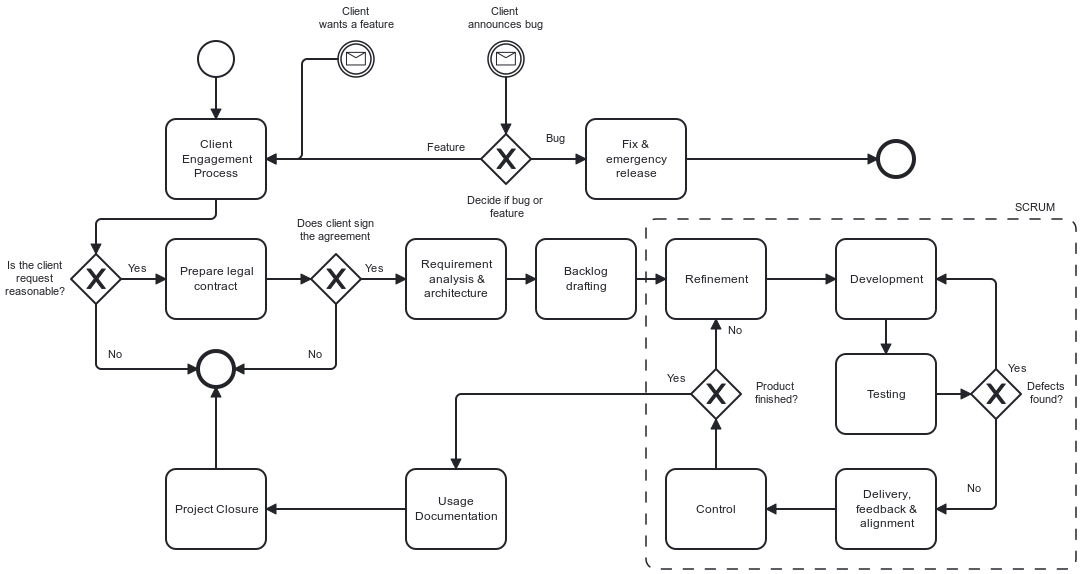
\includegraphics[width=\linewidth]{etc/diagram.png}
\end{figure}
\end{landscape}

\subsection{\process{EngageClient}} % ARNAS

\begin{figure}[H]%[htpb!]
    \centering
    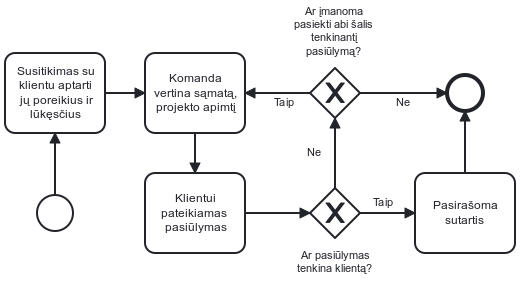
\includegraphics[width=0.75\linewidth]{etc/engage-client.png}
\end{figure}

\begin{processTable}{EngageClient}
    \tikslas{Įvertinti kliento poreikius, rasti kompromisą dėl projekto sąmatos bei apimties ir pasirašyti sutartį}
    \inputs{
        \item \textit{KP}. Kliento poreikiai ir galimybės
        \item \workProd{Experience}
    }
    \outputs{   
        \item \workProd{ResourceEstimates}
        
        \item \workProd{ProjectScope}
        
        \item \workProd{Contract}
    }
    \veiklos{
         \item Projektų vadovas, architektas ir analitikas bendrauja su klientu, aiškinasi jo poreikius sistemai ir vertina kliento galimybes finansuoti tokios sistemos kūrimą. Ši veikla tęsiasi tol, kol įmonės atstovai surenka pakankamai informacijos paruošti klientui pasiūlymą.
    
        \item Projektų vadovas, architektas ir analitikas tarpusavyje įvertina kliento norus ir galimybes ir paruošia sutartį į kurią įeina laiko, kainos ir žmogiškųjų ištekliu sąmata bei nusakoma sistemos apimtis. \label{activity:prepare-deal}

        \item Klientui yra pateikiama sutartis. Jei klientas yra patenkintas sutarties sąlygomis pereinama prie sutarties pasirašymo \ref{activity:sign}. Klientas gali nesutikti su sutarties sąlygomis. Tokiu atveju klientas pateikia naujus poreikius ir dar kartą vykdoma veikla \ref{activity:prepare-deal}. Jei abi šalys nesugeba rasti kompromiso, procesas gali būti nutrauktas ir darbas su klientu netęsiamas.

        \item Pasirašoma sutartis su klientu. \label{activity:sign}
    }
\end{processTable}

\newpage
\subsection{\process{RA}} % DOMANTAS

\begin{processTable}{RA}
    \tikslas{Nustatomi reikalavimai, kuriuos turi atitikti sistema, atitinkamai suprojektuojama sistema.Surinkti/nustatyti/išvesti? funkcinius ir nefunkcinius reikalavimus}
    Surinkti/nustatyti/išvesti? funkcinius ir nefunkcinius reikalavimus

% Derive technical requirements that the system must meet and design the system accordingly.
    \inputs{
       \item \workProd{Kazkas}
    }
    \outputs{
       \item \workProd{Kazkas}
    }
    \veiklos{
        \item Kazkokia veikla
    }
\end{processTable}

\begin{table}[h!]
\begin{tabular}{p{0.1\textwidth}|p{0.8\textwidth}}
\hline
\textbf{\processId{RA}}    & \textbf{\processName{RA}} \\ \hline
Tikslas & 
Nustatomi reikalavimai, kuriuos turi atitikti sistema, atitinkamai suprojektuojama sistema.
Surinkti/nustatyti/išvesti? funkcinius ir nefunkcinius reikalavimus

Derive technical requirements that the system must meet and design the system accordingly. \\ \hline

Naudojami darbo produktai &
\begin{itemize}
    \item \workProd{ResourceEstimates}
    
    \item \workProd{ProjectScope}
\end{itemize}
\\ \hline
Sukurti darbo produktai &
\begin{itemize}
    \item \workProd{FunReq}
    \item \workProd{NonFunReq}
    \item \workProd{HighLevelArch}
    % Architecture
\end{itemize}
\\ \hline
Veiklos &   
\begin{enumerate}

    \item Identifikuojamos suinteresuotos šalys ir informacijos šaltiniai.
    \item Renkama informacija iš suinteresuotų šalių per interviu ir modeliuojami įmonės
    procesai iš identifikuotų informacijos šaltinių.
    \item Iš surinktos informacijos identifikuojami konkretūs vartotojų poreikiai
    % \item Perform analysis of gathered intel, document concrete user needs (\textit{UN}).
    \item Apibrėžiami funkciniai ir nefunkciniai reikalavimai iš identifikuotų vartotojų poreikių; laiko kainos, žmogiškųjų išteklių sąmatos ir projekto apimties.
    \item Aukšto lygio sistemos architektūra sukuria atsižvelgiant į apibrėžtus funkcinius ir nefunkcinius reikalavimus.
\end{enumerate}
\\ \hline
\end{tabular}

\label{pro/plan}
\end{table}

\newpage

\subsection{\process{DraftBacklog}} % ARNAS

\begin{table}[h!]
\begin{tabular}{p{0.1\textwidth}|p{0.85\textwidth}}

\hline

\textbf{\processId{DraftBacklog}} & \textbf{\processName{DraftBacklog}} \\ 

\hline

Tikslas &
Paversti analizės metu išgrynintus reikalavimus ir sistemos architektūra į panaudos atvejus ir technines užduotis iš kurių būtų sudaromas užduočių sąrašas. \\ 

\hline

Panaudoti darbo produktai & 

\begin{itemize}
    \item \workProd{FunReq}
    \item \workProd{NonFunReq}
    \item \workProd{HighLevelArch}
\end{itemize}

\\ \hline

Sukurti darbo produktai &

\begin{itemize}
    \item \workProd{Backlog}
\end{itemize} \\ 

\hline

Veiklos &

\begin{enumerate}
    \item Architektas kartu su analitiku agreguoja analizės metu surinktus reikalavimus bei aukšto lygio sistemos architektūra į panaudos atvejus ir atskiras technines užduotis. Kiekvienas panaudos atvejis ir techninė užduotis yra detaliai aprašomi
\end{enumerate} \\ 

\hline

\end{tabular}
\label{pro/back}
\end{table}

\newpage
\subsection{PRO/SCRUM. SCRUM CYCLE }

\subsubsection{PRO/REF. Refinement }

\begin{table}[h!]
\begin{tabular}{l|p{0.725\textwidth}}
\hline
\textbf{PRO/REF}        & \textbf{Refinement} \\ \hline
Purpose & Review and refine the backlog of tasks by breaking them into smaller, more manageable parts. Adjust priorities and ensure clarity in the tasks to align with the product goals and decide what and who will execute it this sprint. \\ \hline
Used work products (IN)   &      
\begin{itemize}
    \item \textit{PB}. Project backlog
    \item \textit{SP}. Story points range
    \item \textit{SRR}. Sprint review report
\end{itemize}
\\ \hline
Created work products (OUT) &     
\begin{itemize}
    \item \textit{PB}. Project backlog
    \item \textit{SB}. Sprint backlog
\end{itemize}
\\ \hline
Activities            &   
\begin{enumerate}
    \item The current \textit{PB} with the team is reviewed, focusing on any new \textit{PB} items added.
    \item Large tasks are broken into smaller, atomic tasks.
    \item Clarity in the task descriptions for better understanding and execution are ensured.
    \item The scrum team  estimates the effort required for each task using story points, typically following the Fibonacci sequence.
    \item Tasks based on current goals and resources are reassessed and prioritised, taking into the consideration \textit{SRR}.
    \item Selected tasks for the cycle with total work load fitting into the story points range (\textit{SP}) for the cycle, creating a sprint backlog (\textit{SB}).
    \item Team members plan who will execute each task.  
\end{enumerate}
\end{tabular}
\label{PRO/REF}
\end{table}

\newpage
\subsubsection{PRO/DEV. Development}

\begin{table}[h!]
\begin{tabular}{l|p{0.725\textwidth}}
\hline
\textbf{PRO/DEV}        & \textbf{Development} \\ \hline
Purpose & To implement the tasks listed in the sprint backlog according to the plan. The scrum team focuses on delivering potentially shippable product increments, ensuring the quality and functionality of the features. \\ \hline
Used work products (IN)    &      
\begin{itemize}
    \item \textit{SB}. Sprint backlog
    \item \textit{DR}. Defect report (conditional, if any defects are found int PRO/TEST)
    \item \textit{CODE}. Code-base
\end{itemize}
\\ \hline
Created work products (OUT) &     
\begin{itemize}
    \item \textit{PI}. Product increment 
    \item \textit{CODE}. Updated code-base.
    \item \textit{DOC}. Technical documentation 
\end{itemize}
\\ \hline
Activities            &   
\begin{enumerate}
    \item Each developer develops tasks as defined in the sprint backlog. Time spent on \textbf{2-7} activities must be logged in (\textit{SB}) for future alignment of tasks. 
    \item They write and maintain code following coding standards, updating the code-base (\textit{CODE}). 
    \item They write unit test with the line coverage of 70\% to ensure code quality and functionality, updating the code-base (\textit{CODE}).
    \item When code and unit tests are written, another team member must review the code. If any  changes are requested the processes is repeated from \textbf{2-4}.
    \item Once development is completed, all defects (\textit{DR}) have been addressed, and the code has been approved by another developer, the product increment (PI) for testing is prepared. The task status in the sprint backlog (SB) must be updated to reflect that the task is testable.
    \item Any necessary documentation (\textit{DOC}) must be written as well.
\end{enumerate}
\end{tabular}
\label{PRO/DEV}
\end{table}

\newpage
\subsubsection{PRO/TEST. Testing}

\begin{table}[h!]
\begin{tabular}{l|p{0.725\textwidth}}
\hline
\textbf{PRO/TEST}        & \textbf{Testing} \\ \hline
Purpose & To verify that the product increment meets the defined acceptance criteria and quality standards without breaking something in previous product increments. Testing ensures the product is functional, reliable. \\ \hline
Used work products (IN)    &      
\begin{itemize}
    \item \textit{PI}. Product increment
    \item \textit{DOC}. Technical documentation
    \item \textit{SB}. Sprint backlog
\end{itemize}
\\ \hline
Created work products (OUT) &     
\begin{itemize}
    \item \textit{DR}. Defect reports
    \item \textit{SB}. Updated sprint backlog
\end{itemize}
\\ \hline
Activities            &   
\begin{enumerate}
    \item Testers must log work done in \textbf{2-6} in sprint backlog (\textit{SB}).
    \item Testers review the product increment (\textit{PI}) against acceptance criteria (from \textit{SB}) and requirements, using \textit{DOC} if necessary.
    \item They perform functional and non-functional testing (e.g. integration, system, performance, and security testing) as per requirements of the tasks.
    \item They conduct regression testing (automated) to ensure new changes do not affect existing functionality.
    \item They update defect reports (\textit{DR}) to reflect the quality status.
    \item If defects are found, the task loops back into the development cycle to address the issues. The tester must change the status of the task to reflect that it is back in development in the sprint backlog (\textit{SB}).
\end{enumerate}
\end{tabular}
\label{quality_assurance_process}
\end{table}

\newpage
\subsubsection{PRO/PD. Partial delivery \& feedback}

\begin{table}[h!]
\begin{tabular}{l|p{0.725\textwidth}}
\hline
\textbf{PRO/PD}        & \textbf{Partial delivery \& feedback} \\ \hline
Purpose & To deliver a  product increment to stakeholders and gather feedback. This process ensures that the product is moving in the right direction and that stakeholder expectations are met. \\ \hline
Used work products (IN)    &      
\begin{itemize}
    \item \textit{PI}. Product increment
    \item \textit{DR}. Defect reports
    \item \textit{PB}. Project backlog
\end{itemize}
\\ \hline
Created work products (OUT) &     
\begin{itemize}
    \item \textit{FD}. Feedback documentation
\end{itemize}
\\ \hline
Activities            &   
\begin{enumerate}
    \item Deliver the product increment (\textit{PI}) to stakeholders for initial feedback.
    \item Present the outcomes of the latest sprint, including the features developed and known issues from \textit{DR}.
    \item Collect feedback from stakeholders regarding the delivered increment and its alignment with their needs. Discuss any gaps, potential improvements, and changes to the     \textit{PB}.
    \item Write feedback documentation (\textit{FD}).
\end{enumerate}
\end{tabular}
\label{partial_delivery_feedback_alignment}
\end{table}

\newpage
\subsubsection{PRO/CONTROL. Control (sprint review \& alignment)}

\begin{table}[h!]
\begin{tabular}{l|p{0.725\textwidth}}
\hline
\textbf{PRO/CONTROL}        & \textbf{Control (sprint review \& alignment)} \\ \hline
Purpose & To review and demonstrate the work completed during the sprint, allowing the team to self-evaluate how the sprint went. Feedback from stakeholders is also considered to assess time management and align on improvements for future scrum cycles. \\ \hline
Used work products (IN)    &      
\begin{itemize}
    \item \textit{PI}. Product increment
    \item \textit{DR}. Defect reports
    \item \textit{SB}. Sprint backlog
    \item \textit{EST}.  Resource, time and cost estimates
    \item \textit{SP}. Story point range
    \item \textit{FD}. Feedback documentation
    \item \textit{PB}. Project backlog
\end{itemize}
\\ \hline
Created work products (OUT) &     
\begin{itemize}
    \item \textit{SRR}. Sprint review report summarising the sprint's outcomes 
    \item \textit{SP}. Updated story point range 
\end{itemize}
\\ \hline
Activities            &   
\begin{enumerate}
    \item The team reflects on the sprint's progress, discussing what went well and what challenges were encountered.
    \item The project managed assesses the actual time spent on tasks compared to the initial estimates to understand the team's time management using sprint backlog (\textit{SB}) logged hours and initial time estimates (\textit{EST}).
    \item Based on \textbf{1-2} and feedback documentation (\textit{FD}), the project manager and scrum team identifies necessary adjustments for the next sprint. This includes updating the project backlog (\textit{PB}), reprioritizing tasks as needed and capturing these changes in the sprint review report (\textit{SRR}), refining the story point range (\textit{SP}).
    \item The project manager closes project if necessary - if no further sprints are required, they transition to usage documentation.
\end{enumerate}
\end{tabular}
\label{control_process}
\end{table}


\newpage
\subsection{\process{CreateManual}}

\begin{processTable}{CreateManual}
    \tikslas{Paruošti produkto naudojimo instrukciją, suprantamą naudotojams}
    \inputs{
        \item \workProd{UserNeeds}
        \item \workProd{UseCases}
        \item \workProd{Product}
    }
    \outputs{
            \item \workProd{Manual}
    }
    \veiklos{
         \item Detaliai aprašomi visi žingsniai kiekvienam panaudos atvejui (\workProdId{UseCases}) naudojant produktą (\workProdId{Product}). \label{CreateManual/1}
        \item Detaliai aprašomos visos produkto (\workProdId{Product}) funkcijos (t.y. kaip jomis pasinaudoti) \label{CreateManual/2}
        \item Iš \ref{CreateManual/1}. ir \ref{CreateManual/2}. sudaromas struktūrizuotas, vientisas dokumentas - \prodWork{Manual}
        \item Atliekama produkto naudojimo instrukcijos (\workProdId{Manual}) validacija - paruoštas dokumentas peržiūrimas kolegų iš kitų padalinių, įsitikinama, jog instrukcija suprantama pirmą kartą produktą (\workProdId{Product}) naudojantiems žmonėms \label{CreateManual/3}
        \item Kol netenkinamas \ref{CreateManual/3}. punktas, atliekami naudojimo instrukcijos pakeitimai
        }
\end{processTable}

\begin{figure}[h]
    \centering
    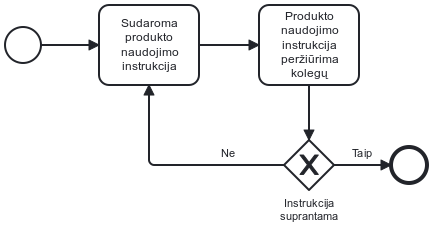
\includegraphics[width=0.75\linewidth]{etc/diagrams/Manual.png}
\end{figure}
% --------------------------------------------------------------------
\newpage
\subsection{\process{CloseProject}}
\begin{processTable}{CloseProject}
    \tikslas{Užbaigti projektą, perduoti paruoštą naudojimui produktą klientams}
    \inputs{
        \item \workProd{Product}
    	\item \workProd{Contract}
    	\item \workProd{Backlog}
    	\item \workProd{TechDocs}
    	\item \workProd{Manual}
    }
    \outputs{
        \item \workProd{Warranty}
        \item \workProd{Experience}
    }
    \veiklos{
         \item Įsitikinama, jog visos užduočių sąraše (\workProdId{Backlog}) numatytos užduotys yra įgyvendintos
        \item Atliekami sutartyje (\workProdId{Contract}) numatyti produkto (\workProdId{Contract}) perdavimo klientui darbai
        \item Klientui perduodama \prodWork{Manual}
        \item Klientui perduodama \prodWork{TechDocs}
        \item Sudaroma ir pasirašoma \prodWork{Warranty}, kurioje numatomas garantinio aptarnavimo laikotarpis
    	\item Atliekama vidinė komunikacija apie užbaigtą projektą. Projekto vadovas dalinasi projekto eiga, priimtais kritiniais sprendimais ir rezultatais. Taip kaupiama \prodWork{Experience} 
    	\item Kol nesibaigia sutartyje (\workProdId{Contract}) numatytas adaptacinis laikotarpis, klientams teikiama techninė pagalba
    }
\end{processTable}

\begin{figure}[!h]
    \centering
    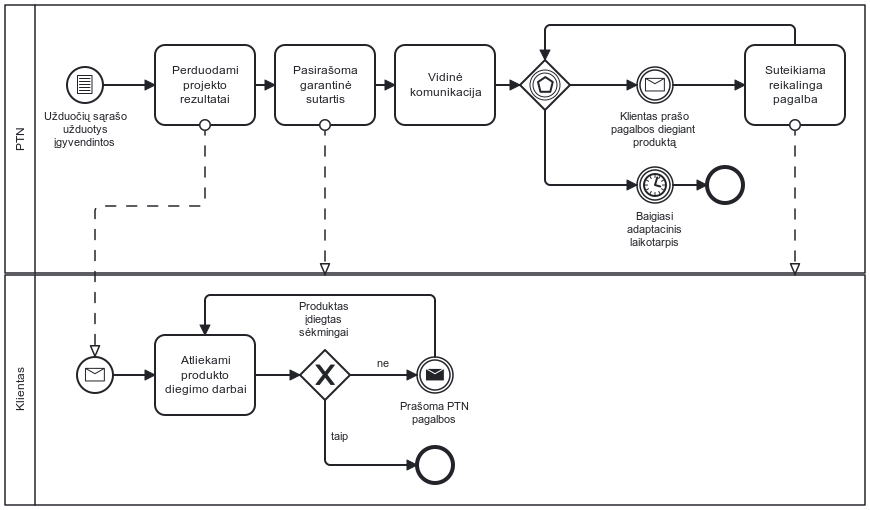
\includegraphics[width=0.8\linewidth]{etc/diagrams/projectClosure.png}
\end{figure}
\newpage

%----------------------------------------


\subsection{\process{BugFix}}
\begin{processTable}{BugFix}
    \tikslas{Ištaisyti ne dėl kliento kaltės kilusias produkto klaidas}
    \inputs{
        \item \workProd{Product}
    	\item \workProd{TechDocs}
    	\item \workProd{Contract}
    	\item \workProd{Warranty}
    	\item \workProd{Ticket}
    	\item \workProd{Manual}    }
    \outputs{
        \item \workProd{Ticket}
    }
    \veiklos{
        \item Atliekama pirminė užregistruotos klaidos (\workProdId{Ticket}) analizė
	   \item Jei užregistruota klaida (\workProdId{Ticket}):
            \begin{enumerate}[label=\alph*)] 
        		\item kyla dėl produkto (\workProdId{Product}) naudojimo nesilaikant produkto naudojimo instrukcijos (\workProdId{Manual})
        		\item eksploatuojant produktą (\workProdId{Product}) netinkamomis, t.y. neatitinkančiomis techninės dokumentacijos (\workProdId{TechDocs}), sąlygomis
        		\item yra ne klaida, o neegzistuojančio ir -sutartyje- (\workProdId{Contract}) nenumatyto funkcionalumo įgyvendinimo prašymas
        		\item neatitinka garantino aptarnavimo sutartyje (\workProdId{Warranty}) numatytų sąlygų
        		\item yra užregistruota po garantino aptarnavimo sutartyje (\workProdId{Warranty}) numatyto garantinio laikotarpio
            \end{enumerate}
            tuomet užregistruota klaida (\workProdId{Ticket}) nėra taisoma ir šis procesas (\textit{BugFix}) yra užbaigiamas nevykdant tolesnių veiklų
    	\item Atliekama klaidos kilimo priežasties analizė (root cause analysis)
    	\item Kuo įmanoma greičiau ištaisoma klaida ir sukuriama nauja produkto (\workProdId{Product}) versija
    	\item Nauja produkto (\workProdId{Product}) versija perduodama klientams
    	\item Užregistruota klaida (\workProdId{Ticket}) papildoma su klaidą ištaisančia prdoukto (\workProdId{Product}) versija bei klaidos kilimo priežastimi    
    }
\end{processTable}
\newpage

%----------------------------------------

% \begin{processTable}{PrimaryKey}
%     \tikslas{}
%     \inputs{
%        \item \workProd{Kazkas}
%     }
%     \outputs{
%        \item \workProd{Kazkas}
%     }
%     \veiklos{
%         \item Kazkokia veikla
%     }
% \end{processTable}


%----------------------------------------